\documentclass[11pt]{article}
\usepackage[sc]{mathpazo} %Like Palatino with extensive math support
\usepackage{fullpage}
\usepackage[authoryear,sectionbib,sort]{natbib}
\linespread{1.7}
\usepackage[utf8]{inputenc}
\usepackage{lineno}
\usepackage{booktabs}

%%%%%%%%%%%%%%%%%%%%%
% LaTeX packages
%%%%%%%%%%%%%%%%%%%%%
% Please be sparing in your use of additional LaTeX packages, and
% upload any required style files to Editorial Manager with the file
% type "LaTeX ancillary files (.sty, .bst)."

%%%%%%%%%%%%%%%%%%%%%
% Line numbering
%%%%%%%%%%%%%%%%%%%%%
\usepackage{lineno}
% Please use line numbering with your initial submission and
% subsequent revisions. After acceptance, please comment out 
% the commands \usepackage{lineno}, \linenumbers{} 
% and \modulolinenumbers[3] below.

\title{Predator phylogenetic diversity decreases predation rate via antagonistic interactions}

%%%%%%%%%%%%%%%%%%%%%
% Authorship
%%%%%%%%%%%%%%%%%%%%%
% Please remove authorship information while your paper is under review,
% unless you wish to waive your anonymity under double-blind review. 
% Remember to uncomment the information after acceptance.

\author{A. Andrew M. MacDonald$^{1,\ast}$ \\ 
Gustavo Q. Romero$^{1,\dag}$ \\ 
Diane S. Srivastava$^{2,\ddag}$}

\date{}

\begin{document}

\maketitle

\noindent{}1. Biodiversity Research Centre, Department of Zoology, University of British Columbia, Vancouver, British Columbia, V6T1Z4, Canada;

\noindent{}2. Departamento de Biologia Animal, Instituto de Biologia, Universidade Estadual de Campinas (UNICAMP), CP 6109, CEP 13083-970 Campinas, S\~{a}o Paulo, Brazil.

\noindent{}$\ast$ Corresponding author; e-mail: macdonal@zoology.ubc.ca

\noindent{}$\ddag$ ORCIDs: MacDonald, orcid.org/0000-0003-1162-169X; .

\bigskip

\textit{Manuscript elements}: Figure~1, figure~2, table~1, online
appendices~A and B (including figure~A1 and figure~A2). %Figure~2 is to
% print in color.

\bigskip

\textit{Keywords}: Predators, food webs, phylogenies.

\bigskip

\textit{Manuscript type}: Article. 
% Or e-article, note, e-note, natural history miscellany,
% e-natural history miscellany, comment, reply, symposium, or
% countdown to 150.

\bigskip

\noindent{\footnotesize Prepared using the suggested \LaTeX{} 
template for \textit{Am.\ Nat.}}

\linenumbers{}
\modulolinenumbers[3]

\newpage{}

\section*{Abstract}

Predator assemblages can differ substantially in their top-down effects on
community composition and ecosystem function, but few studies have sought to
explain this variation in terms of the phylogenetic diversity (PD) of
predators. When predators show broad overlap in their fundamental niches, a
range of PD may be represented in local predator assemblages. In this case, if
distantly-related predators overlap less in their diet, then predator
assemblages with high PD should consume more of the prey community.
Alternatively, if distantly-related predators show more antagonistic
interactions, predator assemblages with high PD should consume less of the
prey community. Either effect of predator PD on prey mortality could have
cascading effects on the ecosystem functions mediated by prey. We examined
predator PD in macroinvertebrate food webs found in bromeliads, a natural
aquatic mesocosm. We use measures of predator PD to combine three datasets:
observations of predator distribution among bromeliads, experimental feeding
trials, and a manipulation of predator PD. We found that phylogenetic distance
does not predict differences in predator distribution, indicating that a range
of predator PD is found in nature. We did, however, find a tendency for
distantly-related predators to eat different prey, a prerequisite for
synergistic effects of predators on prey mortality. However, our manipulative
experiment showed that increasing predator PD reduced prey mortality,
reflecting antagonistic interactions among more distant predators. These
effects of PD on prey mortality did not translate into effects on ecosystem
function, as measured by rates of decomposition and nitrogen cycling. In
conclusion, the effects of predator PD on the bromeliad food web are primarily
determined by antagonistic predator-predator interactions, rather than habitat
distribution or diet overlap. This study illustrates the potential of a
phylogenetic community approach to understanding food webs.


\newpage{}

\section*{Introduction}

% The journal does not have numbered sections in the main portion of
% articles. Please refrain from using section references such as
% section~\ref{section:CountingOwlEggs}, and refer to sections by name
% (e.g. section ``Counting Owl Eggs'').


Predators can have strong top-down effects, both on community structure
and ecosystem processes \citealt{Estes2011}. The combined effect of
predator species on communities is often stronger or weaker than that
predicted from a study of those same species in isolation
\citealt{Sih1998a, Ives2005}. These non-additive effects occur when
predators interact with each other directly, or via their shared prey
species. For example, predators feed directly on each other (intra-guild
predation), consume the same prey (resource competition) or modify the
behaviour of prey or the other predator species
\citealt{Sih1998a, Griswold2006, Nystrom2001}. These non-additive effects
can be positive or negative. For example, prey may have an induced
defense against one predator which increases (negative non-additive
effect) or decreases (positive non-additive effect) the likelihood of
consumption by a second predator. While there are many possible
mechanisms underlying the effect of predator composition, we lack a
means of predicting \emph{a priori} the strength and direction of this
effect on community structure and ecosystem function.

The phylogenetic relationships among predators could provide a framework for combining different approaches to studyin predator-predator interactions, thus helping us make
predictions about combined effects of predators. A phylogenetic approach to species interactions
extends the measurement of species diversity to include the evolutionary
relationships between species. Relatedness may be a proxy for ecological similarity; very
similar species may compete strongly, and/or may interfere with each
other while very different species may not be able to occur in the same
patch. This approach was first used to interpret observations of
community structure, as ecologists interpreted nonrandom phylogenetic
structure (i.e.~under- or over- dispersion) as evidence for the
processes, such as habitat filtering or competition, which structure
communities \citealt{Webb2002, Cavender-Bares2009}. Recently, this
approach has been applied to manipulative experiments. For example, the
phylogenetic diversity of plant communities is a better predictor of
productivity than either species richness or diversity
\citealt[e.g.][]{Cadotte2009, Cadotte2008, Godoy2014}. In all cases, an
implicit assumption is that increased phylogenetic distance is
associated with increased ecological dissimilarity -- either in the form
of differences in species niches, interactions, or functional traits.
When this is true, high phylogenetic diversity should lead to
complementarity in resource use between species, resulting in increased
ecosystem functioning \citealt{Srivastava2012c}. 

Phylogenetic diversity may be a better predictor of species effects on ecosystem funcitioning than species identity along. For example, studies of
plants have shown that in both experimental \citealt{Cadotte2008} and
natural communities, ecosystem function is
positively related to the phylogenetic diversity of plants. Although
there have been many studies taking a phylogenetic approach to community
ecology and although predators have large effects on many communities,
the phylogenetic diversity of local predator assemblages has rarely been
measured \citealt{Bersier2008, Naisbit2011}. Many studies of phylogeny and
predator traits focus on whole clades, rather than local assemblages
(e.g. \emph{Anolis} lizards \citealt{Knouft2006}, warblers
\citealt{Bohning-Gaese2003}, tree boas \citealt{Henderson2013} and wasps
\citealt{Udriene2005}), making it difficult to connect these results to
predator effects at the scale of a local community. These clade specific
studies often find weak evidence for phylogenetic signal in ecologically
relevant traits. In contrast, studies at the level of the whole
biosphere \citealt{Gomez2010, Bersier2008} demonstrate that related
organisms often have similar interspecific interactions, i.e.~related
predators often consume similar prey. At the local scale, only a few
studies have examined how phylogeny may shape food webs
\citealt{Rezende2009, Cagnolo2011}; these observational studies found that
models containing both relatedness (either from taxonomic rank or
phylogenetic trees) and body size were better at predicting which
predator-prey interactions occurred than models with body size alone. As
observational studies, however, they cannot isolate if it is differences
in predator distribution or diet that leads to a phylogenetic signal in
predator-prey interactions, nor how these interactions affect the whole
community.

Can
phylogeny help us predict how predators will impact community composition and ecosystem functioning? Within a local community, the effect of predator species diversity will
depend on three factors: how predators are distributed among habitats,
how they interact with their prey, and how they interact with each other. To the extent that phylogenetic relationships are
correlated with these three factors they enable us to predict the impact
of predator diversity on communities. For instance, phylogeny could
constrain predator species co-occurrence if more distant phylogenetic
relatives have more distinct fundamental niches, whereas close relatives
are too similar to co-exist \citealt{Webb2002, Emerson2008}. When
predators do co-occur, phylogeny may correlate with their feeding
behavior, such that closely related predators consume similar prey. For
example, diet overlap (shared prey species between predators) will
depend on the feeding traits and nutritional requirements of predators
-- both of which may be phylogenetically conserved. If this is the case,
then predator assemblages with higher phylogenetic diversity will show a
greater range of prey consumed and therefore stronger top- down effects
\citealt{Finke2008a}. In some cases, predator diets may extend to include
other predators, leading to direct negative interactions such as
intraguild predation, which may also have a phylogenetic signal
\citealt{Pfennig2000}. To our knowledge, the relationship of phylogeny to
predator distribution, diet, and intraguild interactions has never been
investigated in a single study.

We tested for the effects of phylogenetic distance on distribution, diet
and interactions of predators living in a natural mesocosm: water
reservoirs found inside bromeliad leaves. Bromeliads (Bromeliaceae) are
flowering plants abundant in the Neotropics. Within this aquatic food
web, damselfly larvae (e.g. \emph{Leptagrion} spp.,
Odonata:Coenagrionidae) are important predators that dramatically reduce
insect colonization \citealt{Hammill2015} and emergence
\citealt{Starzomski2010}, and increase nutrient cycling \citealt{Ngai2006}.
In addition to damselfly larvae, other predators are also found in
bromeliads, including large predaceous fly larvae (Diptera: Tabanidae)
and predatory leeches (Hirudinae:Arhynchobdellida) (see Frank et al.
\citeyearpar{Frank2009}). Many bromeliads contain water and trapped,
terrestrial detritus which supplies nutrients for the bromeliad
\citealt{Reich2003a}. The small size of these habitats permits direct
manipulations of entire food webs, manipulations which would be
difficult in most natural systems. Predators have been shown to have
large top-down effects on ecosystem functions in bromelaids, including
nitrogen uptake by the plant \citealt{Ngai2006}, detrital decomposition
and $CO2$ flux \citealt{Atwood2014, Atwood2013}.
% fix
We tested for a relationship between the distribution, diet and
ecosystem effect of predators and their phylogenetic distance using
observations, lab feeding trials, and manipulative field experiments,
respectively. We observed predator distribution by dissecting a sample
of natural bromeliads. We quantified diet preferences in a series of
no-choice feeding trials. Ecosystem-level effects were measured with a
manipulative experiment, where predators were placed alone or in
combination within standardized communities. In each approach, we test
the hypothesis that greater phylogenetic distance correlates with
greater difference in predator impacts on the bromeliad community:

\begin{enumerate}
\def\labelenumi{\arabic{enumi}.}
\item
  \emph{Distributional similarity}: Closely related predators occur in
  the same habitat patch more frequently than less related predators.
  Alternatively, closely related species may never co-occur.
\item
  \emph{Diet similarity}: Closely related predators will eat similar
  prey at similar rates (in other words, there should be a correlation between the relatedness of two predators and their similarity of their diets). Alternatively, closely related species may have
  evolved different diets to facilitate coexistence.
\item
  \emph{Ecosystem-level effects}: We tested two sets of hypotheses about
  direct and indirect effects of predator combinations on ecosystems,
  predicting:

  \begin{enumerate}
  \def\labelenumii{(\alph{enumii})}
  % \tightlist
  \item
    Closely related predators will have similar effects on the
    community and ecosystem. This will occur if related predators have similar trophic
    interactions (e.g.~predation rate, diet similarity). Our
    single-species treatments allow us to assess the effect of each
    predator both on prey survival and on ecosystem functions.
  \item
    Predator assemblages with higher phylogenetic diversity will have
    synergistic (greater than additive) effects on prey consumption and
    associated ecosystem functions. This will occur if phylogenetic
    distance correlates with increasing trait difference, and if this
    trait difference in turn results in niche complementarity. However,
    at the extreme, different predators may consume each other, thus
    creating antagonistic (less than additive) effects on prey
    consumption. By comparing treatments with pairs of predators to
    treatments that received each predator alone, we are able to
    estimate additive and non-additive effects.
  \end{enumerate}
\end{enumerate}

% Please note that we prefer (\citealt{Xiao2015}) to \citep{Xiao2015},
% since \citep{} inserts a comma after "et al."

\section*{Methods}

\subsection*{Study Design}

We used three empirical approaches to test the hypotheses outlined
above. To test hypothesis 1 (distribution) we sampled bromeliads for
predator species. To test hypothesis 2 (diet similarity), we conducted a
series of laboratory feeding trials. Finally, we tested hypothesis 3
(similarity of community effect and interaction) with a field experiment
in which predators were added to bromeliads containing standardized
communities of prey. This experiment included both single species
treatments and two species treatments; the latter were chosen to create
the widest possible range of phylogenetic diversity.

We included phylogenetic information in our analyses of all three
datasets. We obtained this phylogenetic information first from
classification alone. Next we added information about the age of each
node from ``timetree.org'', an online database of published molecular
time estimates \citealt{Hedges2006}. The timetree online database collects
information from multiple independent phylogenetic studies. These
studies provide independent estimates of the age of the most recent
common ancestor for two lineages. Lineages that diverged a long time ago
have been dated by multiple studies; for such nodes we used the median
age. All internal nodes were dated by at least one study, however data
was unavailable for the youngest nodes (i.e.~tips) of the tree. For
these nodes, either a lack of taxonomic information (e.g.~Tabanidae) or
a lack of phylogenetic study (e.g. \emph{Leptagrion}) prevented more
information from being included. These branches were left unresolved
(i.e., as polytomies) and were all assigned identical, arbitrary and
short branch lengths (15 Mya). The result is a phylogeny that closely
resembles the qualitative, taxonomy-based tree with which we began.
Because the node ages between our major predators (leeches, tabanids and
odonata) are so deep, variation among studies in the estimated age of
these nodes was minor compared to the differences between them.

We conducted all three experiments in Parque Estadual da Ilha do Cardoso
(25\textsuperscript{o} 03' S, 47\textsuperscript{o} 53' W), a 22.5 ha
island off the south coast of S\~ao Paulo state, Brazil. We worked in a
coastal forest (\emph{restinga}) with an understory dominated by
\emph{Quesnelia arvensis} Mez. (Bromeliaceae). \emph{Q. arvensis} is a
large terrestrial bromeliad that catches and holds rainwater
(phytotelmata), accumulating up to 2.8 L of rainwater in a single plant.
Our observational survey found more than 47 species of
macroinvertebrates in these aquatic communities \citealt{Romero2010}, in
25 bromeliads of various sizes. This diversity encompasses multiple
trophic and functional groups. Filter feeders were entirely mosquito
larvae (Diptera:Culicidae); detritivores include shredders
(Diptera:Tipulidae, Trichoptera:Calamoceratidae), scrapers
(Coleoptera:Scirtidae), and collectors (All Diptera:Chironomidae,
Syrphidae, Psychodidae). All these species are prey for a diverse
predator assemblage dominated by at least three species of damselfly
larvae (\emph{Leptagrion} spp., Odonata:Coenagrionidae), two species of
Horse Fly larvae (Diptera:Tabanidae), and two species of leech
(Arhynchobdellida). A lower percentage of predator biomass was composed
of Dytiscid larvae (Coleoptera), midge larvae (Diptera: Ceratopogonidae)
and chironomid larvae (Diptera: Tanypodinae).

\subsection*{Data collection}\label{data-collection}

\subsubsection*{Distributional similarity}

We asked whether closely related predators were found in the same
bromeliads. In 2008, each bromeliad was dissected and washed to remove
invertebrates. We passed this water through two sieves (150 and 850 micrometers),
which removed particulate organic matter without losing any
invertebrates. All invertebrates were counted and identified to the
lowest taxonomic level possible. The body length of all individuals was
measured when possible for small and medium-sized taxa (\textless{} 1cm
final instar) and always for large-bodied taxa (\textgreater{} 1 cm
final instar).

\subsubsection*{Diet Similarity}

To test whether related predators eat similar prey, we fed prey to
predators in laboratory feeding trials. We conducted 314 feeding trials
of 10 predator taxa and 14 prey taxa between March and April 2011. We
included all potential predator-prey pairs present in the experiment
(described below), and attempted to perform all other combinations
whenever possible. However, due to the rarity of some taxa, many
predator-prey pairs were not possible; we tested 56 pairwise
combinations. Most trials were replicated at least five times, but the
number of replicates ranged from 1 to 11. To conduct the trials, we
placed predators together with prey in a 50ml vial, with a stick for
substrate. The only exception was the tabanid larvae, which we placed
between two vertical surfaces to imitate the narrow space found in
bromeliad leaf axils (their preferred microhabitat, necessary for
successful feeding). Generally our trials contained a single predator
and a single prey individual, except in the case of very small prey
(\emph{Elpidium} sp.) or predators (\emph{Monopelopia} sp.) in which
case we increased the density. We recorded whether prey was consumed
after 24 hours. We tested for a relationship between predator similarity and diet similarity with a regression weighted by the number of prey assayed (to correct for unequal numbers of replicates)

\subsubsection*{Community effect experiment}

Our third hypothesis had two parts: (a) how do predator species differ
in their effects on the invertebrate community composition (the number of surviving prey species) and ecosystem processes (rates of detrius consumption and nitrogen cycling)
and (b) do predator combinations show non- additive effects on community
and ecosystem processes, and do these non-additive effects increase or
decrease with phylogenetic distance?

We tested effects of both single and multiple predator species on
community responses with a manipulative experiment where identical prey
communities were exposed to treatments of either a single predator, or
pairs of predators representing increasing phylogenetic diversity. In
this experiment we focused on the four most abundant large predators
found in the community: \emph{Leptagrion andromache} and
\emph{Leptagrion elongatum} (Odonata: Coenagrionidae), a predatory
Tabanid fly (Diptera:Tabanidae:\emph{Stibasoma} sp.) and a predatory
leech. We combined these species in eight treatments: predator-free
control (no predators), each of the four predator species alone (3a) and
pairs of predator species chosen to maximize variation in phylogenetic
distance (3b). Specifically, these pairs were: two congeneric
damselflies (\emph{Leptagrion andromache} and \emph{Leptagrion
elongatum}), two insects (\emph{L. elongatum} and \emph{Stibasoma}), and
two invertebrates (\emph{L. elongatum} and a predatory leech). We used
five replicate bromeliads for each of these 8 treatments (8 treatments,
n=5). This experiment, therefore, allows the estimation of the effect of
each predator species (single-species treatments), as well as the
detection of non-additive effects in predator combinations.

We created bromeliad communities that were as similar as possible to
each other, and also to the average composition of a bromeliad. In
February 2011 we collected bromeliads with a volume between 90 and
200ml, thoroughly washed the plants to remove organisms and detritus,
and soaked them for 12 hours in a tub of water. We then hung all
bromeliads for 48 hours to dry. This procedure was intended to remove
all existing macroinvertebrates; one bromeliad dissected afterwards
contained no insects (a similar technique was used by Romero and
Srivastava \citeyearpar{Romero2010}). We simulated natural detritus
inputs from the canopy by adding a standard mass of dried leaves of the
species \emph{Plinia cauliflora} (Jabuticaba, Myrtaceae; a common
Brazilian tree; 1.5g bromeliad \textsuperscript{-1} $\pm$ 0.02, mean $\pm$ sd).
In order to track the effects of detrital decomposition on bromeliad N
cycling, we enriched these leaves with \textsuperscript{15}N by
fertilizing five plants with 40ml pot\textsuperscript{-1}
day\textsuperscript{-1} of 5g L\textsuperscript{-1} ammonium sulphate
containing 10\% atom excess of \textsuperscript{15}N. After 21 days we
then collected \emph{P. cauliflora} leaves, air-dried until constant
weight, and then soaked them for three days. This procedure removes
excess nutrients from the artificial fertilization. Because some of our
prey species consume fine detritus, not coarse, we also added a standard
amount of dried fine detritus to our bromeliads (0.23g bromeliad
\textsuperscript{-1} $\pm$ 0.02). We separated coarse and fine detritus by
passing water from bromeliads through two sieves (as above for
observational work, 150 and 850 micrometer). We defined ``coarse detritus'' as
anything retained on the 850 micrometer sieve, and ``fine detritus'' as anything
found on the 150 micrometer sieve.

Each bromeliad was stocked with a representative insect community (See
supplementary material). The densities of each prey taxon were
calculated from the observational dataset (Hypothesis 1), using data
from bromeliads of similar size to those in our experiment. We ran this
experiment in two temporal blocks for logistical reasons: three complete
replicates of all treatments were set up on 20 February 2011, and two on
08 March 2011. We first placed the prey species into the bromeliad,
allowed two days for the prey to adjust, then added predators. After 26
days from the beginning of each block, we added the same prey community
a second time to simulate the continuous oviposition that characterizes
the system. We concluded the experiment 43 days from the first addition
of prey (20 April 2011). Throughout the experiment, all bromeliads were
enclosed with a mesh cage topped with a malaise trap and checked daily
for emergence of adults. At the end of the experiment we completely
dissected our bromeliads, collecting all invertebrates and detritus
remaining inside.

We used a substitutive design, maintaining the same predator metabolic
capacity in all replicates (see below). In a substitutive experiment,
all experimental units receive the same ``amount'' of predators --
usually standardized by abundance -- and only species composition
varies. However, when species differ substantially in body size - as in
this experiment - abundance does not standardize the their effects on
the community. We chose to standardize using metabolic capacity instead
(after Srivastava \citeyearpar{Srivastava2009a}). Integrating the
allometric relationship between body size and feeding rate
\citealt{Brown2004, Wilby2005} over all individuals of a species allows
estimates of ``metabolic capacity'', or the potential energy
requirements of a species \citealt{Srivastava2009a}. Metabolic capacity is
equal to individual body mass raised to the power of 0.69 (an
invertebrate-specific exponent determined by Peters
\citeyearpar{Peters1986} for invertebrates and confirmed by Chown et al,
\citeyearpar{Chown2007}); this reflects the nonlinear relationship
between feeding rate and body size across many invertebrate taxa.

To quantify the effect of predators on ecosystem function, at the end of
the experiment we measured five community and ecosystem response
variables: decomposition of coarse detritus, production of fine
particulate organic matter (FPOM), bromeliad growth, uptake of detrital
nitrogen into bromeliad tissue, and survival of invertebrate prey
(emerged adults + surviving larvae). We measured decomposition by once
again passing the bromeliad water through a 850 micrometer sieve, collecting the
retained detritus and determining the mass of this detritus after
oven-drying it at approximately 70\(^\circ\)C. We measured the
production of FPOM by taking the remaining liquid and filtering it on
pre-weighed coffee filters, which were then dried and reweighed. We
measured bromeliad growth as the average increase in length of five
leaves per plant. We tracked the uptake of labeled detrital nitrogen by
analyzing three innermost (closest to meristem) bromeliad leaves at the
end of the experiment. Finally, we quantified the species composition
and survivorship of invertebrate prey by combining counts of emerging
adult insects and surviving larvae.

We measured decomposition by collecting all \emph{Plinia} leaves from
bromeliads; these were oven-dried at 70\(^\circ\)C before their mass was
determined. At the end of experiment, we sampled three new bromeliad
leaves for isotopic (\textsuperscript{15}N) and nitrogen concentration
analyses. These analyses were performed at the Stable Isotope Facility
laboratory (UC Davis, CA, USA) using continuous flow isotope ratio mass
spectrometer (20-20 mass spectrometer; PDZ Europa, Sandbach, England)
after sample combustion to N\textsubscript{2} at 1000C by an on-line
elemental analyzer (PDZ Europa ANCA-GSL).

\subsection*{Data analysis}

We quantified the effect of phylogenetic distance on each of
distributional (Hypothesis 1) and diet (Hypothesis 2) similarity. First,
we calculated phylogenetic distance between each pair of species, then
fit several functions to the relationship between phylogenetic diversity
an either distributional or diet similarity. We used linear, constant,
and several appropriate nonlinear functions (nonlinear, because our
measures of similarity are bounded by 0 and 1; see below). We compared
these models using AIC and generated confidence intervals as appropriate
(parametric or bootstrap for linear and nonlinear, respectively). We
quantified both distributional and diet similarity between predators
using Pianka's index of niche overlap \citealt{Pianka1974}:

\begin{equation}
{ O_{kl}=\dfrac{\sum_i^n{p_{il} p_{ik}}}{\sqrt{\sum_i^n{p_{il}^2} \sum_i^n{p_{ik}^2}}} }
\end{equation}

For each pair of predators, \(p_{ik}\) and \(p_{il}\) represent the
preference of predator \(k\) or \(l\) for resource or habitat \(i\). The
value \(O_{kl}\) represents similarity (in our case, in either
distribution or diet) and ranges from 0 (complete dissimilarity) to 1
(complete similarity). The \(n\) resources represent the different
habitats surveyed for Hypothesis 1 (distributional similarity), or the
different prey species assayed for Hypothesis 2 (diet similarity).
Preference (\(p_{ik}\)) represents the proportion of a predator's total
metabolic capacity found in a particular bromeliad (Hypothesis 1); or
the proportion of feeding trials in which it ate a particular prey
(Hypothesis 2). We used a Mantel test to test for correlation between the phylogenetic distance matrix
and dissimilarity in either predator distribution or diet preferences.

We tested hypothesis 3 with a field experiment. We divided the analysis of this experiment into three parts: quantifying
the effect of phylogenetic distance on prey community similarity, on
community and ecosystem responses, and on non-additive effects of
predator combinations. First, we compared the four treatments with
single predator species by calculating the similarity in species
composition (Pianka's index) between surviving prey communities and
relating this to the phylogenetic distance between predators with a
linear regression. If predator feeding choices are phylogenetically
conserved, that diet similarity will decline with increasing
phylogenetic distance.

Second, we measured five community and ecosystem responses, testing in
turn the effect of predator presence, number, species identity, and
finally phylogenetic diversity. To test for an effect of predator
presence, we compared the control treatment (predators absent) with the
mean responses of all seven treatments that did contain predators. To
test for an effect of predator species number (one or two predators), we
compared the means of all single-species treatments with the means of
all two-species treatments. To test for an effect of predator identity,
we compared all four single-species treatments. Finally, to test for an
effect of predator combinations we compared all two-species treatments
(3 pairs total). We analyzed each of these of these orthogonal
comparisons with one-way ANOVA.

In our third and final analysis we quantified the non-additive effect of
predator species on our responses. We calculated this effect as the
difference between the response in bromeliads with both predator species
(n=5) and the mean response in bromeliads with either one of these two
predator species (n=5 for each predator species). We generated bootstrap
confidence intervals for these non-additive effects; confidence
intervals that do not overlap zero indicate a significant non-additive
effect of a predator combination. We used R version 3.2.0 \citealt{rcore}
for most calculations, and two packages: picante \citealt{picante} for
calculating phylogenetic distances matrices, and vegan \citealt{vegan} for
distance metrics.

\section*{Results}

\subsection*{Hypothesis 1: similarity in distribution}

We did not find any significant relationship between predator
co-occurrence in bromeliads (measured as Pianka's index of niche
overlap) and the phylogenetic distance between them (Figure \ref{fig:phylo_niche_overlap}a,
F\textsubscript{1,89}=2.39, p=0.13). This indicates that all 14 predator
species have roughly similar habitat distributions at the level of the
bromeliad. Indeed we often found multiple predator species co-occurring
in the same bromeliads (mean 4.4 $\pm$ 2.9 predator species per plant). A
Mantel test also found no evidence of correlation between differences
among predators in habitat use, and phylogenetic distance (correlation
-0.16, p = 0.81, 999 permutations). We were able to sample a wide range
of phylogenetic relatedness, including two groups of congenerics -- two
species of \emph{Bezzia} sp. (Diptera:Ceratopogonidae) and three species
of \emph{Leptagrion} sp. (Odonata:Coenagrionidae). There were also two
groups of confamilials -- three species of Tabanidae and two species of
Empididae, all Diptera. Deeper divisions were also present: three
families of Diptera were represented by a single predator species each
(Dolichopodidae, Corethrellidae and Chironomidae) and the deepest
taxonomic divide was between all insects present and the predatory
leeches (Arhynchobdellida:Hirudinidae).

\subsection*{Hypothesis 2: Similarity in diet}

Phylogenetically distant predators differed in their preference of prey
species, as measured by the niche overlap index (Fig 1b, regression
weighted by the number of prey assayed, F\textsubscript{1,26}=5.98,
p=0.022). However a Mantel test found no evidence of correlation between
dissimilarity in diet and phylogenetic distance among predators
(correlation -0.27, p = 0.90, 999 permutations).

\subsection*{Hypothesis 3: similarity in top-down effects}

We analyzed our five univariate response variables from the manipulative
experiment by dividing them into four separate and orthogonal tests:
predator presence, predator number, predator species identity and,
increasing predator phylogenetic diversity. Across all four tests, we
saw the strongest responses for total prey survivorship (Table \ref{tab:pdeffects}). Prey
survivorship was halved when predators were present (Figure \ref{fig:ortho_pred_effect}a, Table \ref{tab:pdeffects}). Despite the decline in diet similarity with phylogenetic distance
(Question 2), the variation in predator feeding behaviour did not
translate into a significant differences in the composition of prey
species surviving the manipulative experiment (Fig 1c,
F\textsubscript{1,4}=0.71, p=0.45, distance measured as Bray-Curtis
dissimilarity). Although single predator species had similar effects on
survivorship (Figure \ref{fig:ortho_pred_effect}c, Table \ref{tab:pdeffects}), combinations of predators with higher
phylogenetic diversity showed a significant increase in total prey
survivorship (Figure \ref{fig:ortho_pred_effect}d). That is, more phylogenetically diverse predator
combinations caused less prey mortality. Interestingly, these effects on
prey surviorship did not result in a change in the processing of
detritus (measured either as reduction in coarse detritus or production
of fine detritus), bromeliad growth or nitrogen cycling (Table \ref{tab:pdeffects}).

We tested for non-additive effects of predator phylogenetic diversity
with bootstrap confidence intervals. When we compared the actual effects
of predator combinations with those expected from the mean of each
single-species treatment, we found that predator pairs with the greatest
phylogenetic diversity had the highest prey survival. Whereas effects of
\emph{L. andromache} and \emph{L. elongatum} in combination were quite
similar to the effect of either alone, when \emph{L. elongatum} was
placed in the same plant as either a \emph{Stibasoma} larva or leeches,
on average five more prey individuals (18\% of total prey community)
survived till the end of the experiment (Figure \ref{fig:non_additive}; Tabanid, p = 0.006,
Leech, p = 0.026). Once again, this effect on invertebrate density did
not in turn create a significant difference in other response variables.

%%%%%%%%%%%%%%%%%%%%%%%%%%%%%%%%%%%%%%%%%%%555

\section*{Discussion}

\section*{Discussion}

We found that in our bromeliad system the phylogenetic distance between
predators had variable importance. The phylogenetic distance between
predators was unrelated to co-occurrence (Hypothesis 1). However, as
phylogenetic distance between predator species increased, diet overlap
decreased by 20\% (Hypothesis 2). Interestingly, these apparent diet
preferences in the lab did not generate a difference in species
composition of surviving prey in the field (Hypothesis 3a). Greater
phylogenetic diversity caused an increase in prey survival (i.e.~a
decrease in predation); phylogenetically distant pairs of predators that
co-occurred in bromeliads had less impact on prey than expected from
their performance in isolation (Hypothesis 3b).

\subsection*{Phylogenetic distance and similarity in distribution}

Phylogenetic distance between predators did not explain overlap in
habitat distribution. This similarity in distribution could be caused by
two processes: low habitat variability among bromeliads, or low
variability in preference of predators for different habitats. A
concurrent observational study (AAMMD, unpublished) showed that
bromeliads vary widely in abiotic conditions, size, detritus amount and
prey community; therefore it seems unlikely that low patch variation
explains the lack of pattern. It appears instead that predators do not
possess any strong phylogenetically-conserved preferences for different
habitat characteristics, showing instead very generalist habitat
preferences. This is not surprising, given that these organisms live in
small, fluctuation-prone habitats. As a group, predatory invertebrates
in bromeliads do not show more sensitivity to bromeliad size or drought
than other invertebrates \citealt{Amundrud2015}. The co-occurrence of
predator species within bromeliads suggests that antagonistic
interactions among predators do not limit species distributions.
Additionally, it appears that predator species are able to co-occur in
many different combinations, creating a range of phylogenetic
diversities within bromeliads. This suggests that the range of
phylogenetic diversity we tested in our experiment was realistic.

\subsection*{Phylogenetic distance and similarity in diet}

We observed a negative relationship between phylogenetic distance and
overlap in diet as measured by laboratory feeding trials. This suggests
that there is a phylogenetic signal to predator feeding traits. For
example, damselflies are visual predators that engulf prey whole using
specialized mouthparts; they are gape-limited and cannot eat prey that
are too large. Leeches, in contrast, lack eyes but are able to pierce
prey and consume them without swallowing. Damselflies showed a much
stronger preference for culicid larvae than did leeches, whereas leeches
were slightly better able to kill and consume scirtids. Culicid larvae
are free swimming in the water column, and are therefore easily captured
by engulfing predators, whereas scirtid larvae crawl on surfaces and are
difficult to remove. Although in this study such feeding traits are
phylogenetically structured, in other studies functional traits can be
more important than phylogeny \emph{per se} to a predator's diet: Moody
\citeyearpar{Moody1993} found that unrelated decapod species which were
morphologically similar were also functionally similar. Similarly,
Rezende et al. \citeyearpar{Rezende2009} found that both body size and
phylogeny determined the food web ``compartment'' (shared predator-prey
interactions) of predators in a marine foodweb.

\subsection*{Phylogenetic distance and non-additive effects}

We found that the presence of predators reduced prey survival, but that
this reduction was less for phylogenetically-diverse combinations of
predators. This was contrary to our hypothesis that more distant
predators would show an increase in prey capture via complementarity.
\emph{L. andromache} did not produce an antagonistic (i.e.~less than
additive) effect in combination with \emph{L. elongatum}, whereas the
two more phylogenetically diverse combinations (\emph{L. elongatum} with
the Tabanid or leech) did. \emph{Leptagrion} species may not distinguish
between conspecifics and congenerics. In predicting a synergistic
non-additive effect of predators, we were imagining an outcome much like
those reported by Nilsson et al. \citeyearpar{Nilsson2006c}. They found
that stoneflies caused prey to move into habitats where fish predators
could consume them, increasing total predation (a synergistic effect,
caused by a phylogenetically distinct predator). Our results are more
consistent with those of Finke and Denno \citeyearpar{Finke2005}, who
found that combinations with two insect predators had a higher
per-capita effect on leafhopper prey than combinations with an insect
and a spider. That is, more phylogenetically diverse combinations of
predators showed less predation on lower trophic levels.

When \emph{L. elongatum} occurred with more distantly related predators,
prey survivorship was greater than expected. This non-additive effect
may have been due to a reduction in predation by odonates in the
presence of non-odonate predators. Odonates have been shown to be
sensitive to chemical cues \citealt{Barry2014} or tactile cues
\citealt{Atwood2014} of potential predators, which causes a decrease in
feeding rate. For example, a different species of bromeliad damselfly --
\emph{Mecistogaster modesta} Selys -- reduces predation when it is
housed with Dytiscid adults \citealt{Atwood2014}. If there is a
phylogenetic signal to the chemical cues released by predators,
individuals of one species might be unable to distinguish close
relatives (congenerics in our case) from conspecifics. One limitation of
our approach is that all phylogenetic diversity treatments contained one
species in common, \emph{Leptagrion elongatum}. It is possible that this
species is more sensitive to the presence of other predators, and
therefore shows a larger effect in combination than would other species
in this community. However, this is the most common predator in this
community and our results indicate that its top-down effects are likely
to be frequently reduced by the presence of other predators.

In our experiment we did not see any effect of predator presence, nor of
increasing predator phylogenetic diversity, on ecosystem function
(defined here as Nitrogen cycling, detritus decomposition and bromeliad
growth). This was contrary to our predictions based on the results of
Ngai and Srivastava \citeyearpar{Ngai2006}, who found that adding
predators to a community increased Nitrogen cycling. While we did
observe differences in prey consumption, the resulting changes in
detritivore density did not cause differences in decomposition of
detritus. This difference may be due to leaf traits of the
\emph{restinga} vegetation. In \emph{restinga} vegetation, leaves are
generally extremely tough and waxy, whereas in rainforests, leaves tend
to be softer -- with the result that, in \emph{restinga}, invertebrates
are unable to consume leaves directly. Several lines of evidence support
this assertion. Romero and Srivastava \citeyearpar{Romero2010} studied
the effects of the spider \emph{Corinna} gr. \emph{rubripes}
(Corinnidae) on bromeliad ecosystems. This spider has no effect on the
composition of detritivore communities, nor on decomposition rates, but
increases nitrogen content in bromeliads, probably by depositing feces
or the carcasses of terrestrial prey. This indicates that
\emph{restinga} bromeliads may derive less of their nitrogen from
terrestrial detritus, but may benefit more from terrestrial inputs. A
separate experiment (GQ Romero, pers comm) supports the hypothesis that
lower decomposition in \emph{restinga} is due to plant traits. This
second experiment contrasted decomposition caused by invertebrates and
bacteria with that caused by bacteria alone (by comparing bagged
detritus enclosed in coarse vs fine mesh). The experiment used two
species of detritus: leaves from a rainforest tree, and leaves from a
\emph{restinga} tree. Invertebrates only caused an increase in
decomposition for the rainforest tree, not the \emph{restinga} tree.

\section*{Conclusion}

In most natural communities, multiple predator species co-occur and
often simultaneously affect prey species. By combining an observational
study, laboratory trials, and a field experiment that controlled number
and phylogenetic diversity of predators we have shown that phylogenetic
relatedness of species can help predict some aspects of lower trophic
level responses. An approach based on phylogenetic diversity offers an
organizing framework around which to compare diverse datasets on the
distribution, trophic interactions and combined effect of multiple
predator species, to predict the top-down effect of diverse predator
assemblages.

%%%%%%%%%%%%%%%%%%%%%
% Acknowledgments
%%%%%%%%%%%%%%%%%%%%%
% You are encouraged to remove the Acknowledgments section while
% your paper is under review (unless you wish to waive your anonymity
% under double-blind review) if the Acknowledgments reveal your
% identity. If you remove this section, you will need to add it back
% in to your final files after acceptance.

\section*{Acknowledgments}

%% from a google doc

\newpage{}

\renewcommand{\thesection}{\Alph{section}}

\section*{Online Appendix A: Supplementary Figures}

% Subsection numbering is permitted (but by no means necessary) in 
% online appendices. Please note that if you have sections (thus Online
% Appendix A, B, and C), these will become three separate online PDFs.
% You may wish to consolidate these into one PDF (hence one section,
% divided into subsections as necessary). Please reset counters for
% each such section. 

\renewcommand{\theequation}{A\arabic{equation}}
% redefine the command that creates the equation number.
\renewcommand{\thetable}{A\arabic{table}}
\setcounter{equation}{0}  % reset counter 
\setcounter{figure}{0}
\setcounter{table}{0}

\subsection*{Fox--dog encounters through the ages}

The quick red fox jumps over the lazy brown dog. The quick red fox has 
always jumped over the lazy brown dog. The quick red fox began jumping 
over the lazy brown dog in the 19th century and has never ceased from so 
jumping, as we shall see in figure~\ref{Fig:Jumps}.

[Figure A1 goes here.]

[Figure A2 goes here.]

\newpage{}

\section*{Online Appendix B: Additional Methods}

\renewcommand{\theequation}{B\arabic{equation}}
% redefine the command that creates the equation number.
\setcounter{equation}{0}  % reset counter 
\renewcommand{\thetable}{B\arabic{table}}
\setcounter{figure}{0}
\setcounter{table}{0}

\subsection*{Measuring the height of fox jumps without a meterstick}

Pellentesque ac nibh placerat, luctus lectus non, elementum mauris. 
Morbi odio velit, eleifend ut hendrerit vitae, consequat sit amet 
nulla. Pellentesque porttitor vitae nisl quis tempus. Pellentesque 
habitant morbi tristique senectus et netus et malesuada fames ac 
turpis egestas. Praesent ut nisi odio. Vivamus vel lorem gravida 
odio molestie volutpat condimentum et arcu. 

\begin{equation}
{ \frac{1}{N_k-1} \sum \limits_{t=1}^{N_k} (M_{tjk} - \bar{M}_{jk})^2}
\end{equation}

\subsection*{Quantifying the brownness of the dog}

Pellentesque eu nulla odio (\citealt{Xiao2015,CookEtAl2015}). Nulla 
aliquam porta metus, quis malesuada orci faucibus quis. Suspendisse nunc 
magna, tristique sit amet sollicitudin nec, elementum et lacus. Sed 
vitae elementum mi. In hac habitasse platea dictumst. Etiam eu tortor 
elit. Sed ac tortor purus. Aliquam volutpat, odio sit amet posuere 
pretium, dolor ex interdum ante, sed luctus quam eros ac nulla. 

\begin{equation}
{ (\sum \limits_{p=1}^P {n_{sp}})^{-1}\sum \limits_{p=1}^P {n_{sp}Q_{p}}}
\end{equation}

\newpage{}

%%%%%%%%%%%%%%%%%%%%%
% Bibliography
%%%%%%%%%%%%%%%%%%%%%
% You can either type your references following the examples below, or
% compile your BiBTeX database and paste the contents of your .bbl file
% here. The amnatnat.bst style file should work for this---but please
% email the journal office at amnat at uchicago dot edu if you run into
% any hitches with it!
% The list below includes sample journal articles, book chapters, and
% Dryad references.


\bibliographystyle{amnatnat}
\bibliography{refs-thesis}
% \begin{thebibliography}{}

% \bibitem[{Cook et~al.(2015)Cook, Collaborator, and Expert}]{CookEtAl2015}
% Cook, O.~E., G.~H. Collaborator, and A.~Q. Expert. 2015.
% \newblock Data from: Template and guidelines for using \LaTeX{} 
% in \textit{The American Naturalist}.
% \newblock American Naturalist, Dryad Digital Repository, 
% http://dx.doi.org/10.5061/dryad.XYZAB.

% \bibitem[{Davis et~al.(2011)Davis, Brakora, and Lee}]{DavisEtAl2011}
% Davis, E.~B., K.~A. Brakora, and A.~H. Lee. 2011.
% \newblock Evolution of ruminant headgear: a review.
% \newblock Proceedings of the Royal Society B 278:2857--2865.

% \bibitem[{Inglis et~al.(2011)Inglis, Roberts, Gardner, and Buckling}]{Ing11}
% Inglis, R.~F., P.~G. Roberts, A.~Gardner, and A.~Buckling. 2011.
% \newblock Spite and the scale of competition in \textit{Pseudomonas
%   aeruginosa}.
% \newblock American Naturalist 178:276--285.

% \bibitem[{Lemod\`{e}le et~al.(2007)Lemodele, Kapitelschreiber, 
% and Exemplar}]{LemKapEx07}
% Lemod\`{e}le, P.-Q., A.~B. Kapitelschreiber, and C.~D.~E. Exemplar. 2007.
% \newblock An exemplary instance of chapters in books.
% \newblock Pages 231--245 \emph{in} J.-P. \'{E}crivain and M.~A. 
% Term\'{e}szettud\'{o}s, eds. Inspiring Instances of Brilliant Writing. 
% Truth Pudding Press, Fond du Lac, WI.

% \bibitem[{Xiao et~al.(2015)Xiao, McGlinn, and White}]{Xiao2015}
% Xiao, X., D.~J. McGlinn, and E.~P. White. 2015.
% \newblock A strong test of the maximum entropy theory of ecology.
% \newblock American Naturalist 185:E705--E80.

% \end{thebibliography}

\newpage{}

\section*{Tables}
\renewcommand{\thetable}{\arabic{table}}
\setcounter{table}{0}

\begin{table}[h]
\caption{Predator diversity effects on community and ecosystem
variables. We measured five community-level variables: total prey
survival (both emerged adults and surviving larvae; see Figure \ref{fig:ortho_pred_effect}), the
breakdown of coarse detritus (decomposition), the production of fine
particulate organic matter (FPOM), the cycling of nitrogen, and the
growth of the bromeliad itself. We contrast treatments in our
experimental design in four ways: comparing treatments with predators to
those without (``Predator Presence''), contrasting predator species
(``Identity''), comparing predator communities of 1 or 2 species
(``Richness''), and considering the effects of phylogenetic distance
between predators (``Pairwise PD''). Values are slope $\pm$ standard error
and * = p \textless{} 0.05, from ANOVA}
\label{tab:pdeffects}
\centering
\begin{tabular}{rrrrr}

\toprule 
Response                & Predator Presence               & Identity                         & Richness                      & Pairwise PD             \\ 
\midrule
Total prey survival   & -7.37 $\pm$ 2.45               & 2.00 $\pm$ 2.07              & 2.05 $\pm$ 1.46              & 0.01 $\pm$ 0.00                 \\
                      & F\textsubscript{1,10} = 9.07*  & F\textsubscript{3,16} = 0.60 & F\textsubscript{1,5} = 1.96  & F\textsubscript{1,13} = 7.64*   \\
Decomposition (g)     & 0.01 $\pm$ 0.02                & -0.01 $\pm$ 0.03             & -0.01 $\pm$ 0.02             & 0.00 $\pm$ 0.00                 \\
                      & F\textsubscript{1,10} = 0.47   & F\textsubscript{3,15} = 1.29 & F\textsubscript{1,5} = 0.21  & F\textsubscript{1,13} = 0.40    \\
FPOM (g)              & -0.06 $\pm$ 0.09               & -0.06 $\pm$ 0.11             & 0.18 $\pm$ 0.07              & -0.00 $\pm$ 0.00                \\
                      & F\textsubscript{1,10} = 0.46   & F\textsubscript{3,15} = 0.28 & F\textsubscript{1,5} = 6.19  & F\textsubscript{1,13} = 1.45    \\
Bromeliad growth      & -0.79 $\pm$ 1.10               & -1.08 $\pm$ 1.62             & 0.59 $\pm$ 0.84              & 0.00 $\pm$ 0.00                 \\
                      & F\textsubscript{1,10} = 0.51   & F\textsubscript{3,16} = 0.96 & F\textsubscript{1,5} = 0.49  & F\textsubscript{1,12} = 1.29    \\
Nitrogen cycling      & -5.69 $\pm$ 4.03               & -0.22 $\pm$ 8.66             & 3.97 $\pm$ 5.63              & -0.00 $\pm$ 0.01                \\
                      & F\textsubscript{1,10} = 2.00   & F\textsubscript{3,16} = 1.84 & F\textsubscript{1,5} = 0.50  &  F\textsubscript{1,13} = 0.15   \\
\bottomrule
\end{tabular}
\bigskip{}
\\
% {\footnotesize Note: .}
\end{table}

\newpage{}

%%%%%%%%%%%%%%%%%%%%%
% Figure legends
%%%%%%%%%%%%%%%%%%%%%
% Please include all figure legends in a separate section at the end of 
% the document. If you use \label{} and \ref{} to refer to your figures,
% these can still work even if you comment out the %includegraphics{}
% line. If you refer to figures as "fig. 1" (etc.) manually, the
% legends can also appear simply as paragraphs.
% For submission, please upload the relevant figure files separately to
% Editorial Manager; Editorial Manager should insert them at the end of
% the PDF automatically.
% Figure legends should be concise, though they can be longer than the
% titles of tables.

\section*{Figure legends}

\begin{figure}[htbp]
% 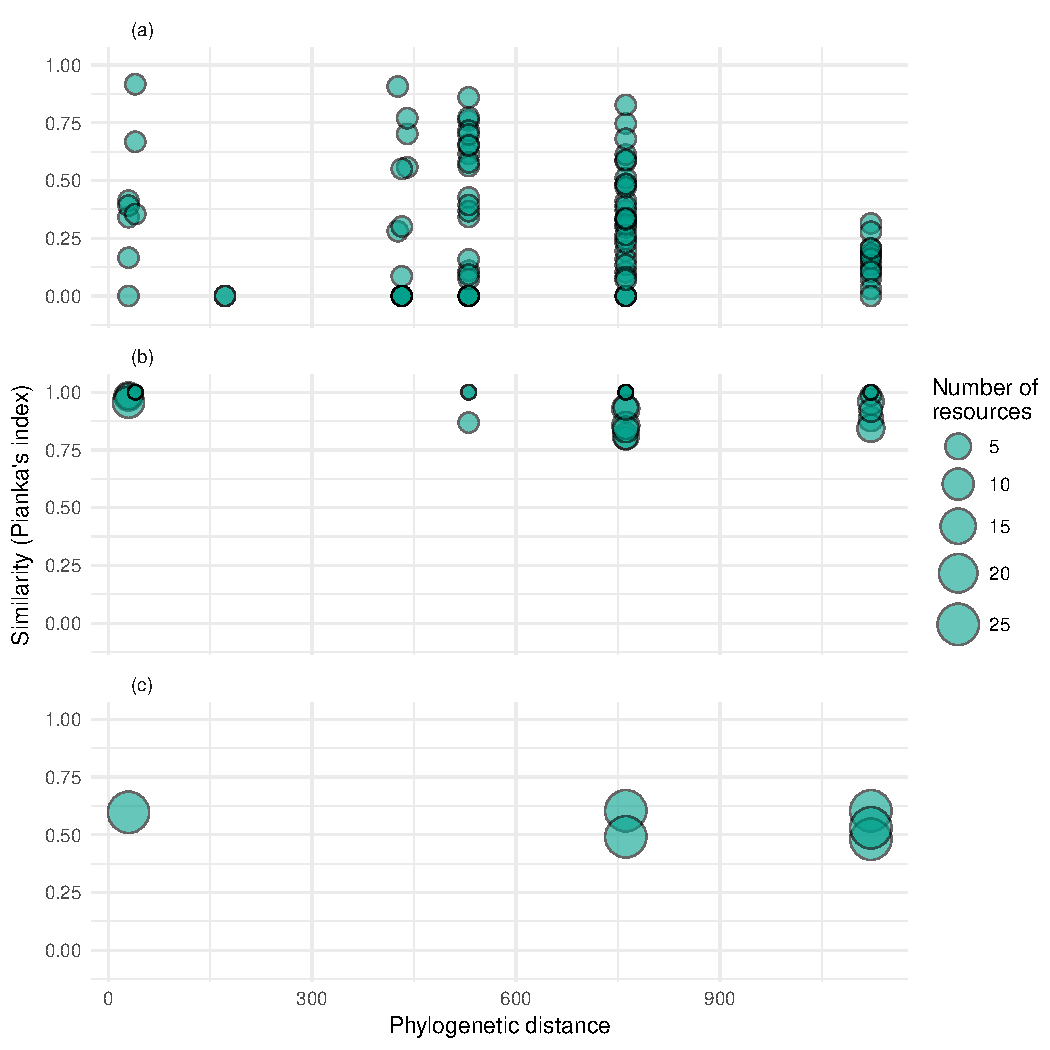
\includegraphics[width=5.5in]{figures/FIG_1.pdf}
\caption[Phylogenetic distance between predators as a
predictor of niche overlap among predators and impacts on prey
composition.]{Phylogenetic distance between predators as a
predictor of niche overlap among predators and impacts on prey
composition. Our measures of niche overlap were: (a) distribution among
bromeliads and (b) diet preferences. We also show the effect of
phylogenetic distance between predators on (c) community dissimilarity
of surviving prey (Bray-Curtis dissimilarity). We measured
distributional similarity (a) by counting all predators in 25
bromeliads, estimating their total metabolic capacity, and calculating
niche overlap (Pianka's index) among all pairs of species. We measured
diet preferences (b) for a subset of these predators by offering them
various prey in no-choice trials, and again calculated niche overlap
among them. Finally, we measured community composition of surviving prey
(c) at the end of an experiment in which predators were placed in
bromeliads with standardized prey communities. For (a) and (b) we used
Pianka's index of niche overlap (1 = complete niche overlap) and tested
various nonlinear and linear models (see Appendix) of the relationship
between this index and phylogenetic distance. Solid lines show
significant model fit, and dashed lines show bootstrap 95\% quantiles.}
\label{fig:phylo_niche_overlap}
\end{figure}


\begin{figure}[htbp]
% 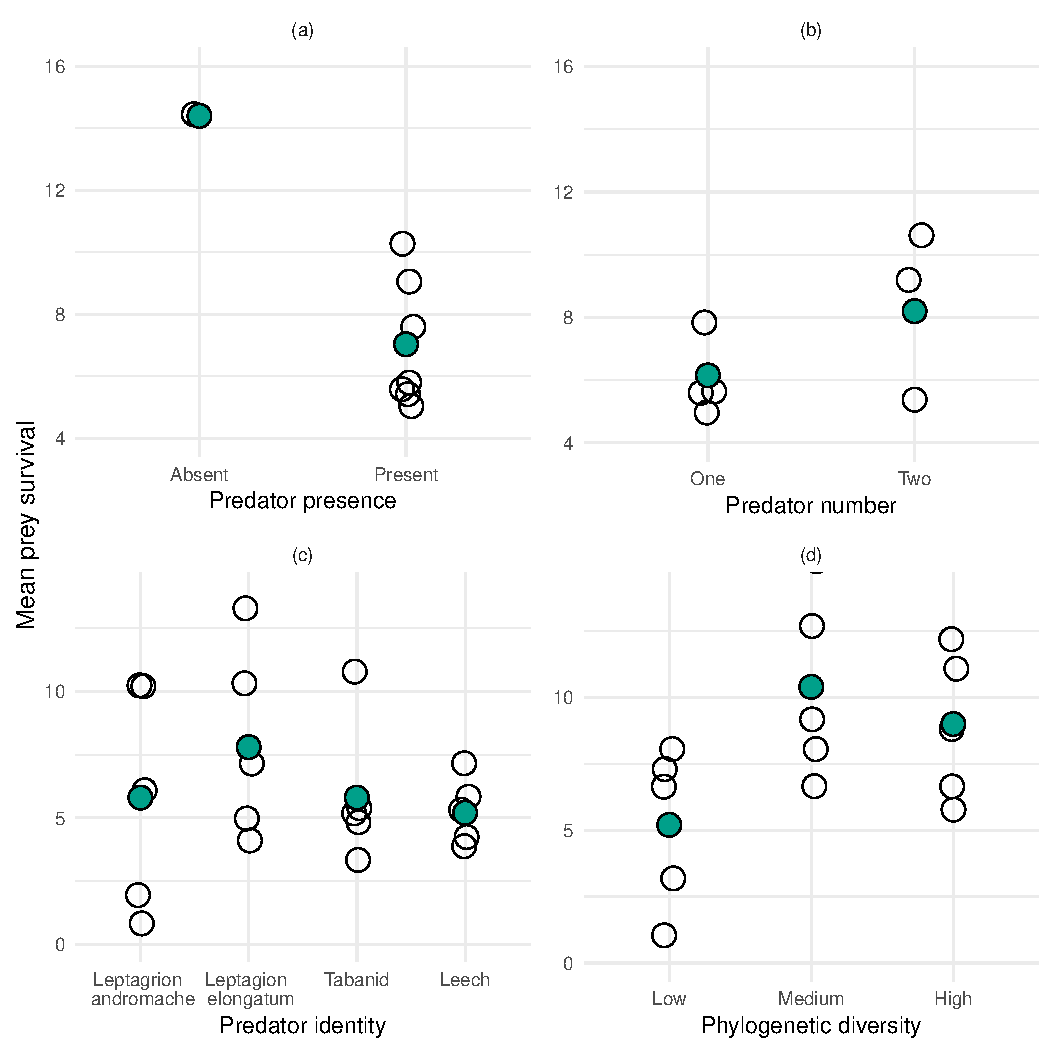
\includegraphics[width=5.5in]{figures/FIG_2.pdf}
\caption[Orthogonal comparisons of the effect of predators on
prey survival. ]{Orthogonal comparisons of the effect of predators on
prey survival. We show the effects of predator presence (a), and then
within predator present treatments the effects of predator species
number (b). Within treatments with one predator species, we show effects
of predator identity (c). Within treatments with two predator species,
we show the effect of increasing phylogenetic diversity (d, arranged in
order of increasing phylogenetic distance: Low = \emph{L. andromache} +
\emph{L. elongatum}, Medium = \emph{L. elongatum} + tabanid, High =
\emph{L. elongatum} + leech). Shaded dots represent grand means for each
group; unshaded dots are either treatment means (2a and 2b, n = 5) or
individual bromeliads (2c and 2d). Points are jittered horizontally
slightly to reveal all datapoints.}
\label{fig:ortho_pred_effect}
\end{figure}


\begin{figure}[htbp]
% 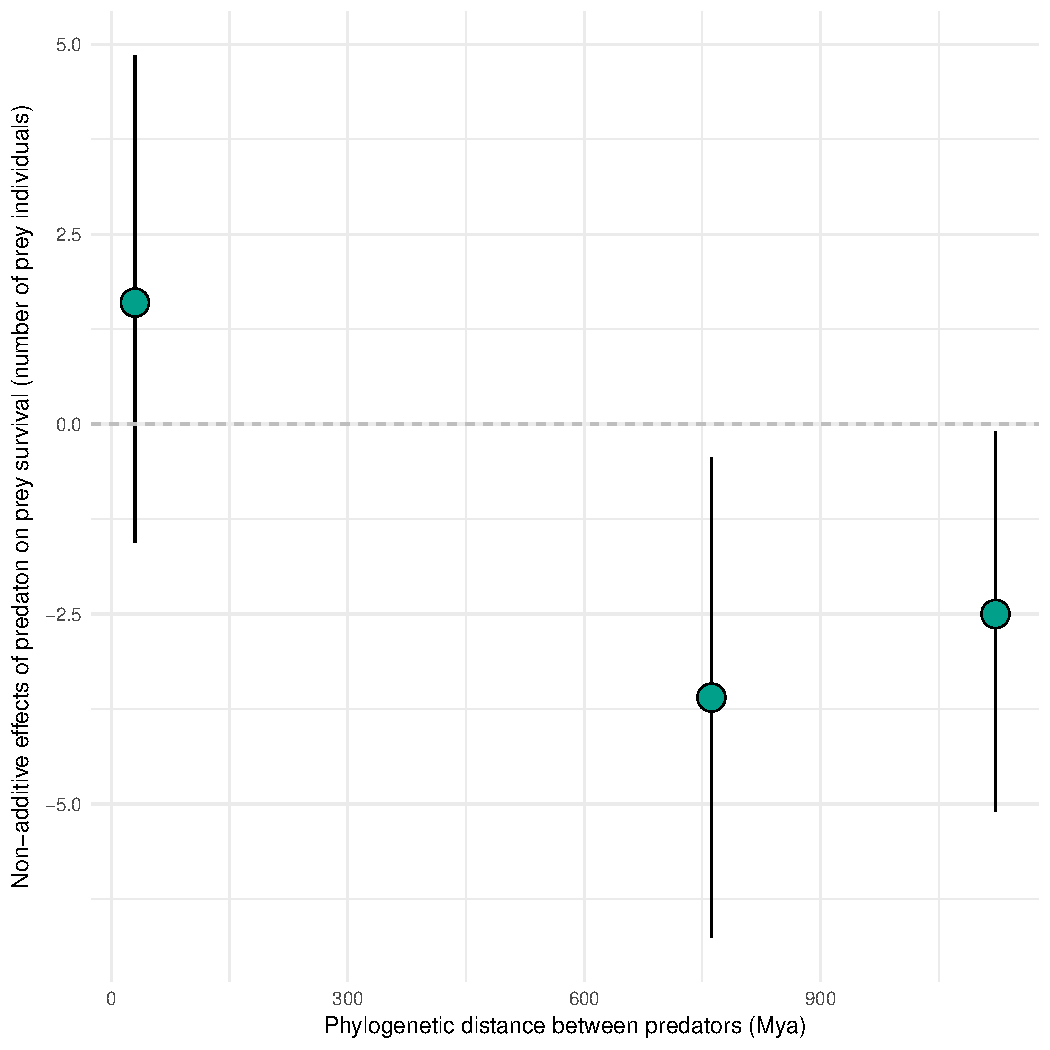
\includegraphics[width=5.5in]{figures/FIG_3.pdf}
\caption[Non-additive effects of predator combinations on prey
decrease with increasing phylogenetic distance between predators]{Non-additive effects of predator combinations on prey
decrease with increasing phylogenetic distance between predators. A
difference of 0 indicates that two-predator treatments resulted in no
more prey mortality than would be expected from simply averaging
single-predator treatments. A negative difference indicates that
two-predator treatments resulted in less mortality than expected. Error
bars represent bootstrap 95\% confidence intervals.}
\label{fig:non_additive}
\end{figure}


% \subsection*{Online figure legends}

% \renewcommand{\thefigure}{A\arabic{figure}}
% \setcounter{figure}{0}

% \begin{figure}[h!]
% %\includegraphics{jumps20m}
% \caption{\textit{A}, the quick red fox proceeding to jump 20~m straight 
% into the air over not one, but several lazy dogs. \textit{B}, the quick 
% red fox landing gracefully despite the skepticism of naysayers.}
% \label{Fig:Jumps}
% \end{figure}

% \begin{figure}[h!]
% %\includegraphics{jumps-nr-okapi}
% \caption{The quicker the red fox jumps, the likelier it is to land near 
% an okapi. For further details, see \citet{LemKapEx07}.}
% \label{Fig:JumpsOk}
% \end{figure}

% \renewcommand{\thefigure}{B\arabic{figure}}
% \setcounter{figure}{0}

\end{document}
